\documentclass[tikz,border=10pt]{standalone}
\usepackage{tikz}
\usepackage{amsmath}
\usetikzlibrary{shapes.geometric, arrows, positioning, fit, calc, shadows.blur, backgrounds}

\begin{document}
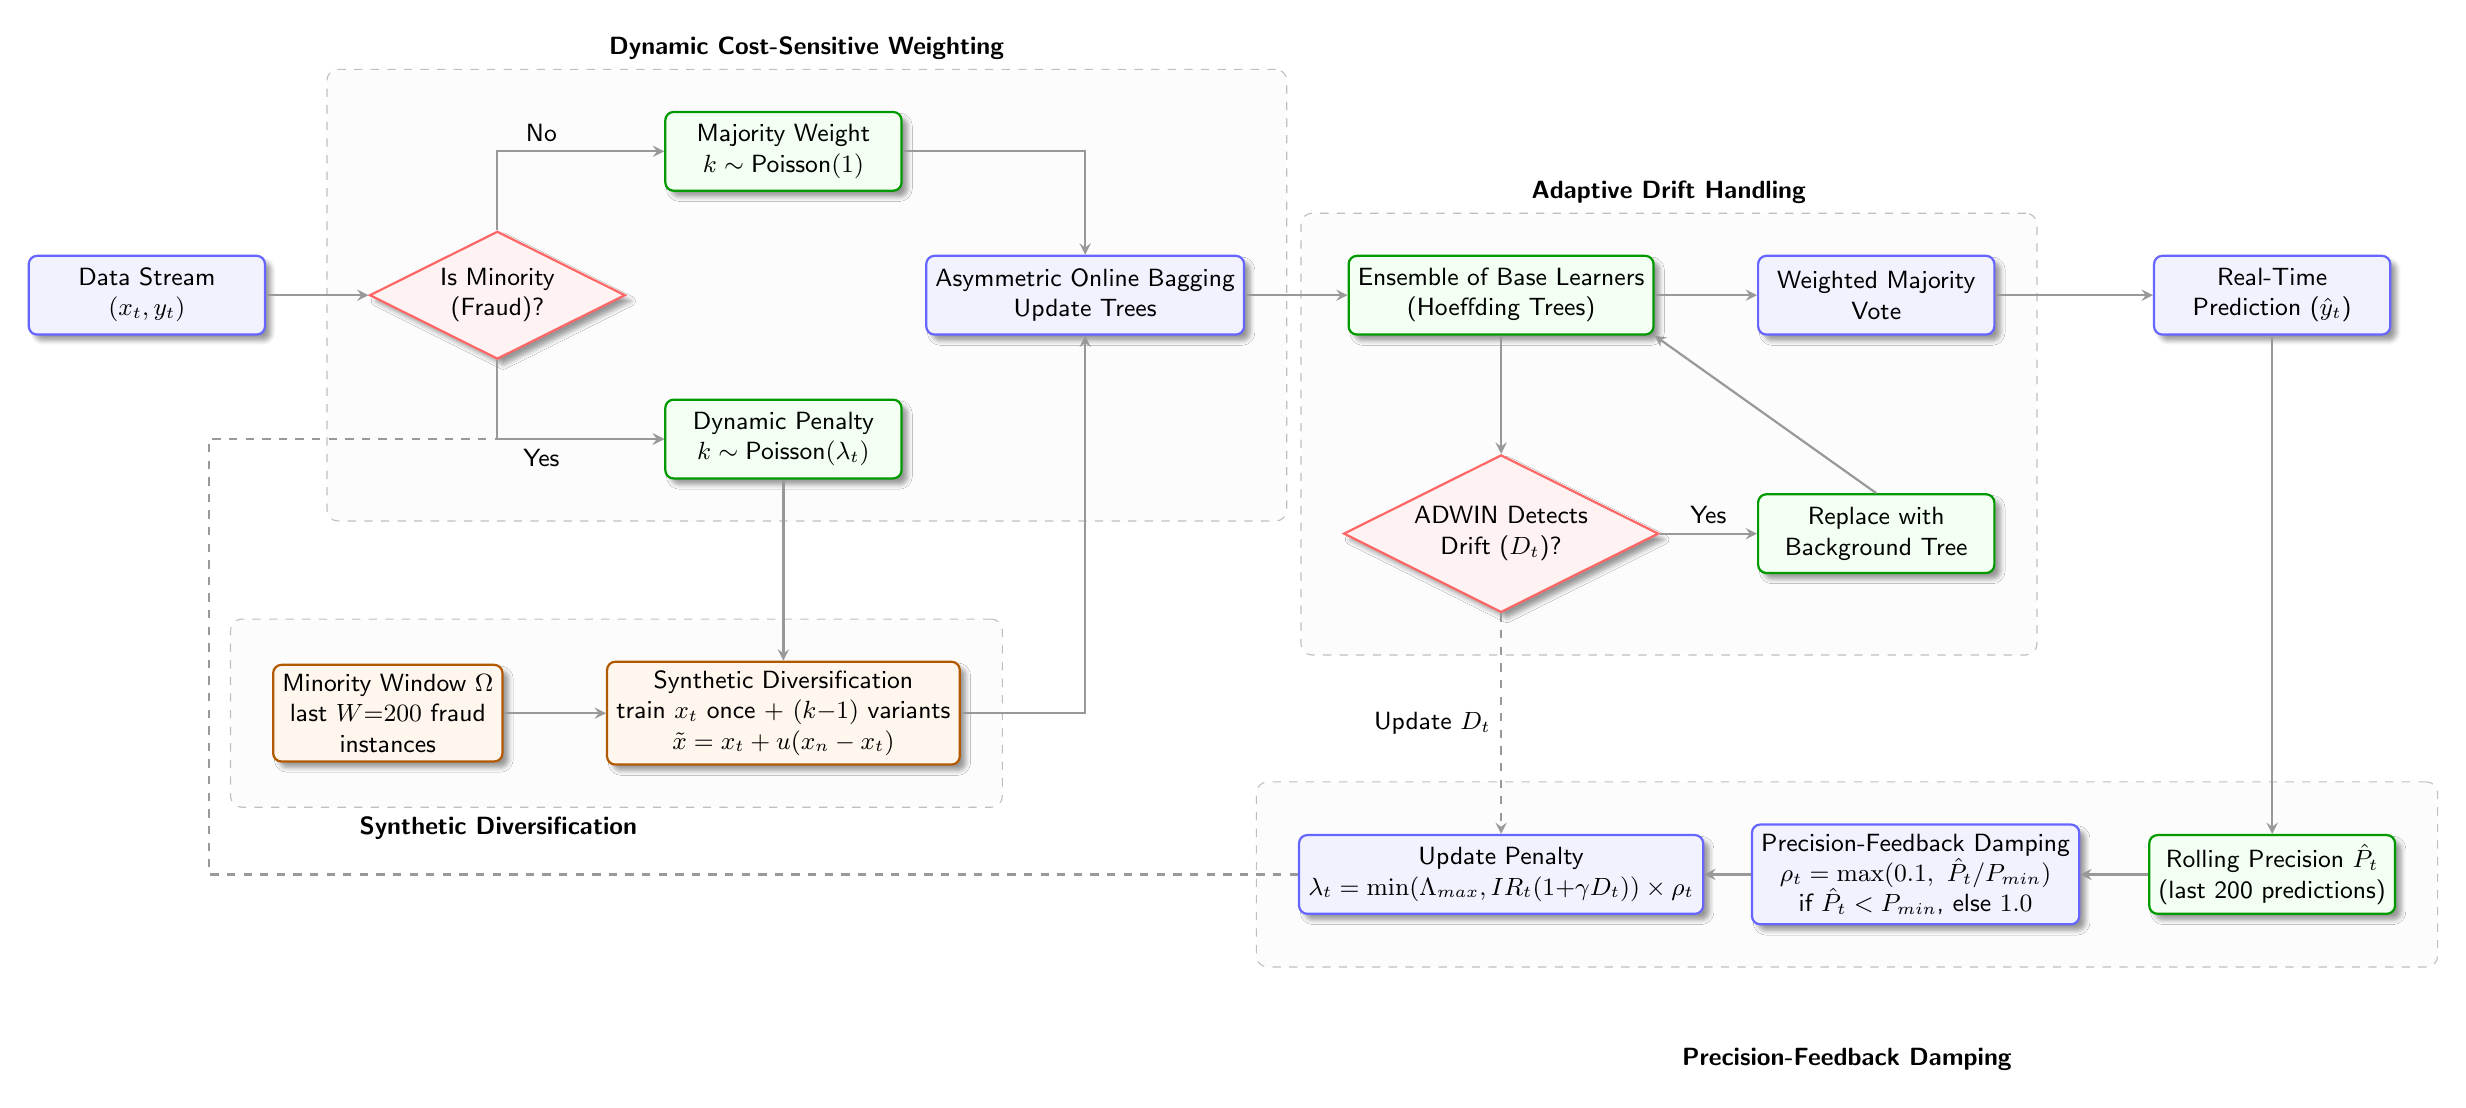
\begin{tikzpicture}[
    >=stealth,
    node distance=1.4cm and 1.5cm,
    font=\sffamily\small,
    box/.style={rectangle, draw=blue!60, fill=blue!5, thick, minimum width=3cm, minimum height=1cm, align=center, rounded corners=3pt, blur shadow={shadow blur steps=5}},
    process/.style={rectangle, draw=green!60!black, fill=green!5, thick, minimum width=3cm, minimum height=1cm, align=center, rounded corners=3pt, blur shadow={shadow blur steps=5}},
    synth/.style={rectangle, draw=orange!70!black, fill=orange!7, thick, minimum width=2.9cm, minimum height=1cm, align=center, rounded corners=3pt, blur shadow={shadow blur steps=5}},
    decision/.style={diamond, aspect=2, draw=red!60, fill=red!5, thick, align=center, inner sep=2pt, blur shadow={shadow blur steps=5}},
    arrow/.style={->, thick, draw=gray!80},
    dashed_arrow/.style={->, thick, dashed, draw=gray!80},
    group/.style={rectangle, draw=gray!50, fill=gray!2, dashed, rounded corners, inner sep=15pt}
]

% ---- Row 1: Cost-sensitive weighting ----
\node[box] (stream) {Data Stream \\ $(x_t, y_t)$};

\node[decision, right=1.3cm of stream] (check_class) {Is Minority\\ (Fraud)?};

\node[process, above right=0.9cm and 1.3cm of check_class] (maj_weight) {Majority Weight\\ $k \sim \text{Poisson}(1)$};
\node[process, below right=0.9cm and 1.3cm of check_class] (min_weight) {Dynamic Penalty\\ $k \sim \text{Poisson}(\lambda_t)$};

\path (maj_weight) -- (min_weight) coordinate[midway] (mid_weights);
\node[box, right=1.8cm of mid_weights] (bagging) {Asymmetric Online Bagging\\ Update Trees};

\node[process, right=1.3cm of bagging] (ensemble) {Ensemble of Base Learners\\ (Hoeffding Trees)};

\node[box, right=1.3cm of ensemble] (aggregation) {Weighted Majority\\ Vote};

\node[box, right=2.0cm of aggregation] (prediction) {Real-Time\\ Prediction ($\hat{y}_t$)};

% ---- Row 2: Synthetic diversification (directly below Row 1, left side) ----
\node[synth, below=2.3cm of min_weight] (diversify) {Synthetic Diversification\\ train $x_t$ once $+$ $(k{-}1)$ variants\\ $\tilde{x} = x_t + u(x_n - x_t)$};

\node[synth, left=1.3cm of diversify] (window) {Minority Window $\Omega$\\ last $W{=}200$ fraud\\ instances};

% ---- Row 3: Adaptive drift handling (below ensemble) ----
\node[decision, below=1.5cm of ensemble] (adwin) {ADWIN Detects\\ Drift ($D_t$)?};
\node[process] (replace) at (aggregation |- adwin) {Replace with\\ Background Tree};

% ---- Row 4: Precision feedback + penalty update (bottom row) ----
\node[box, below=2.8cm of adwin] (calc_lambda) {Update Penalty\\ $\lambda_t = \min(\Lambda_{max}, IR_t(1{+}\gamma D_t)) \times \rho_t$};
\node[box] (damping) at ($(aggregation |- calc_lambda) + (0.5cm, 0)$) {Precision-Feedback Damping\\ $\rho_t = \max(0.1,\ \hat{P}_t / P_{min})$\\ if $\hat{P}_t < P_{min}$, else $1.0$};
\node[process] (precision) at (prediction |- calc_lambda) {Rolling Precision $\hat{P}_t$\\ (last 200 predictions)};

% ---- Connections: Row 1 ----
\draw[arrow] (stream) -- (check_class);
\draw[arrow] (check_class.north) |- (maj_weight.west) node[pos=0.75, above, xshift=-0.5cm] {No};
\draw[arrow] (check_class.south) |- (min_weight.west) node[pos=0.75, below, xshift=-0.5cm] {Yes};

\draw[arrow] (maj_weight.east) -| (bagging.north);
\draw[arrow] (min_weight.south) -- (diversify.north);
\draw[arrow] (window) -- (diversify);
\draw[arrow] (diversify.east) -| (bagging.south);

\draw[arrow] (bagging) -- (ensemble);
\draw[arrow] (ensemble) -- (aggregation);
\draw[arrow] (aggregation) -- (prediction);

% ---- Connections: Row 3 ----
\draw[arrow] (ensemble) -- (adwin);
\draw[arrow] (adwin.east) -- node[above] {Yes} (replace.west);
\draw[arrow] (replace.north) -- (ensemble.south east);

% ---- Connections: Row 4 (feedback loop) ----
\draw[arrow] (prediction.south) -- (precision.north);
\draw[arrow] (precision.west) -- (damping.east);
\draw[arrow] (damping.west) -- (calc_lambda.east);
\draw[dashed_arrow] (calc_lambda.west) -| ($(window.west) + (-0.8,0)$) |- (min_weight.west);
\draw[dashed_arrow] (adwin.south) -- node[left] {Update $D_t$} (calc_lambda.north);

% Background Groups
\begin{scope}[on background layer]
\node[group, fit=(maj_weight) (min_weight) (check_class) (bagging), label={[shift={(0,0)}]above:\textbf{Dynamic Cost-Sensitive Weighting}}] (group1) {};
\node[group, fit=(diversify) (window), label={[shift={(-1.5cm,0)}]below:\textbf{Synthetic Diversification}}] (group1b) {};
\node[group, fit=(ensemble) (adwin) (replace), label={[shift={(0,0)}]above:\textbf{Adaptive Drift Handling}}] (group2) {};
\node[group, fit=(precision) (damping) (calc_lambda), label={[shift={(0cm,-0.9cm)}]below:\textbf{Precision-Feedback Damping}}] (group3) {};
\end{scope}

\end{tikzpicture}
\end{document}
